\documentclass[xetex,mathserif,serif]{beamer}
\usepackage{polyglossia}
\setdefaultlanguage[babelshorthands=true]{russian}
\usepackage{minted}
\usepackage{tabu}

\useoutertheme{infolines}

\usepackage{fontspec}
\setmainfont{FreeSans}
\newfontfamily{\russianfonttt}{FreeSans}

\setbeamertemplate{blocks}[rounded][shadow=false]
\setbeamercolor*{block title example}{fg=green!50!black,bg=green!20}
\setbeamercolor*{block body example}{fg=black,bg=green!10}

\setbeamercolor*{block title alerted}{fg=red!50!black,bg=red!20}
\setbeamercolor*{block body alerted}{fg=black,bg=red!10}

\tabulinesep=0.7mm

\title{Обзор библиотек логирования}
\author[Юрий Литвинов]{Юрий Литвинов \newline \textcolor{gray}{\small\texttt{yurii.litvinov@gmail.com}}}

\date{16.03.2017г}

\begin{document}
	
	\frame{\titlepage}
	
	\section{Введение}

	\begin{frame}
		\frametitle{Логирование}
		\begin{itemize}
			\item Отладочный вывод --- дешёвая альтернатива отладке
			\begin{itemize}
				\item Иногда быстрее вставить отладочную печать, чем проходить отладчиком
				\item Иногда отладчик недоступен или бесполезен
				\begin{itemize}
					\item Многопоточные и распределённые приложения
					\item Встроенные системы
				\end{itemize}
			\end{itemize}
			\item Post-mortem-анализ
			\begin{itemize}
				\item "Отладочный вывод" должен работать и на развёрнутой системе
				\item И выводить не в консоль
				\item И обеспечивать информацию о контексте
			\end{itemize}
			\item Проблемы:
			\begin{itemize}
				\item Scrolling blindness
				\item Замедление приложения
			\end{itemize}
			\item Примерно 4\% кода типичных проектов связано с логированием
		\end{itemize}
	\end{frame}

	\section{Log4j}

	\begin{frame}
		\frametitle{Apache Log4j 2, основные понятия}
		\begin{description}
			\item [Logger] --- штука, которая может что-то куда-то выводить (на самом деле, производить логирующие события)
			\item [LoggerConfig] --- управляет поведением логгера
			\item [LogManager] --- создаёт, хранит и выдаёт по запросу логгеры
			\item [Filter] --- фильтрует логирующие события, говоря, надо или не надо их куда-то выводить
			\item [Appender] --- на самом деле выводит информацию куда-то (в файл, на консоль, в системный лог и т.д.)
			\item [Layout] --- говорит, в каком формате и какую информацию о событии следует выводить
		\end{description}
		\begin{center}Вся конфигурация --- иерархическая!\end{center}
	\end{frame}

	\begin{frame}
		\frametitle{Архитектура}
		\begin{center}
			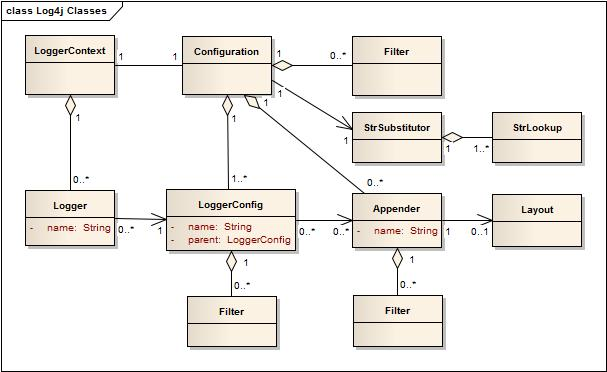
\includegraphics[width=0.9\textwidth]{log4jClasses.jpg}
		\end{center}
	\end{frame}

	\begin{frame}[fragile]
		\frametitle{Пример}
		\begin{minted}{java}
import org.apache.logging.log4j.LogManager;
import org.apache.logging.log4j.Logger;
 
public class HelloWorld {
    private static final Logger logger 
            = LogManager.getLogger("HelloWorld");
    public static void main(String[] args) {
        logger.info("Hello, World!");
    }
}
		\end{minted}
\end{frame}

	\begin{frame}[fragile]
		\frametitle{Пример конфигурации}
		\begin{minted}{xml}
<?xml version="1.0" encoding="UTF-8"?>
<Configuration monitorInterval="30">
  <Appenders>
    <Console name="Console" target="SYSTEM_OUT">
      <PatternLayout pattern=
          "%d{HH:mm:ss.SSS} [%t] %-5level %logger{36} - %msg%n"/>
    </Console>
  </Appenders>
  <Loggers>
    <Root level="error">
      <AppenderRef ref="Console"/>
    </Root>
  </Loggers>
</Configuration>
		\end{minted}
\end{frame}

	\begin{frame}
		\frametitle{Куда это писать}
		Log4j ищет конфигурации в следующих местах в следующем порядке:
		\begin{itemize}
			\item Системное свойство "log4j.configurationFile" (указывается при запуске опцией -D)
			\item log4j2-test.properties в classpath
			\item log4j2-test.yaml или log4j2-test.yml в classpath
			\item log4j2-test.json или log4j2-test.jsn в classpath
			\item log4j2-test.xml в classpath
			\item log4j2.properties в classpath
			\item log4j2.yaml или log4j2.yml в classpath
			\item log4j2.json или log4j2.jsn в classpath
			\item log4j2.xml в classpath
			\item Иначе используется DefaultConfiguration, которая выводит на консоль
		\end{itemize}
	\end{frame}

	\begin{frame}[fragile]
		\frametitle{Уровни и маркеры}
		Уровни логирования: \textbf{TRACE}, \textbf{DEBUG}, \textbf{INFO}, \textbf{WARN}, \textbf{ERROR}, \textbf{FATAL}, \textbf{OFF}

		Маркеры --- способ тонкой настройки информации, которую хочется выводить. Пример:
		\begin{minted}{java}
private static final Marker SQL_MARKER 
        = MarkerManager.getMarker("SQL");

private static final Marker QUERY_MARKER 
        = MarkerManager.getMarker("SQL_QUERY")
                       .setParents(SQL_MARKER);
...
logger.debug(QUERY_MARKER, "SELECT * FROM {}", table);
		\end{minted}
\end{frame}

	\begin{frame}[fragile]
		\frametitle{Синтаксис конфигурации (1)}
		\begin{minted}{xml}
<?xml version="1.0" encoding="UTF-8"?>
<Configuration>
  <Properties>
    <Property name="name1">value</property>
    <Property name="name2" value="value2"/>
  </Properties>
  <Filter type="type" ... />
  <Appenders>
    <Appender type="type" name="name">
      <Filter type="type" ... />
    </Appender>
    ...
  </Appenders>
		\end{minted}
\end{frame}

	\begin{frame}[fragile]
		\frametitle{Синтаксис конфигурации (2)}
		\begin{minted}{xml}
  <Loggers>
    <Logger name="name1">
      <Filter type="type" ... />
    </Logger>
    ...
    <Root level="level">
      <AppenderRef ref="name"/>
    </Root>
  </Loggers>
</Configuration>
		\end{minted}
\end{frame}

	\begin{frame}
		\frametitle{Appenders}
		\begin{description}
			\item [Console] --- выводит в SYSTEM\_OUT или SYSTEM\_ERR
			\item [File] --- выводит в указанный файл
			\item [RollingFile] --- выводит в указанный файл, создавая новые файлы и удаляя старые при необходимости
			\begin{itemize}
				\item TriggeringPolicy --- когда переходить к следующему файлу и что-то делать с предыдущими
				\begin{itemize}
					\item При запуске, по времени, по размеру, по дате/часу
				\end{itemize}
				\item RolloverStrategy --- что делать с файлами
				\begin{itemize}
					\item По шаблону (хитро), с указанием максимума хранимых файлов, кого удалять, сжатие логов
				\end{itemize}
			\end{itemize}
			\item [Ещё штук 20]
		\end{description}
	\end{frame}

	\begin{frame}[fragile]
		\frametitle{Пример конфигурации}
		\begin{footnotesize}
			\begin{minted}{xml}
<?xml version="1.0" encoding="UTF-8"?>
<Configuration name="MyApp">
  <Appenders>
    <RollingFile name="RollingFile" 
        fileName="logs/app.log"
        filePattern=
          "logs/$${date:yyyy-MM}/app-%d{MM-dd-yyyy}-%i.log.gz">
      <PatternLayout>
        <Pattern>%d %p %c{1.} [%t] %m%n</Pattern>
      </PatternLayout>
      <Policies>
        <TimeBasedTriggeringPolicy />
        <SizeBasedTriggeringPolicy size="250 MB"/>
      </Policies>
    </RollingFile>
  </Appenders>
  ...
</Configuration>
			\end{minted}
		\end{footnotesize}
\end{frame}

	\begin{frame}
		\frametitle{Patterns}
		\begin{tabu} {| X[0.2 l p] | X[1 l p] |}
			\tabucline-
			\everyrow{\tabucline-}
			c/logger   & Имя логгера                                    \\
			C/class    & Имя класса, который вывел сообщение            \\
			d/date     & Дата и время                                   \\
			p/level    & Уровень логирующего события (TRACE, INFO, ...) \\
			t/thread   & Имя потока, в котором произошло событие        \\
			m/message  & Собственно, сообщение из программы             \\
			n          & Перевод строки                                 \\
			marker     & Полное имя маркера                             \\
			L/line     & Строка, где вызвали логгер                     \\
			highlight  & Штука, позволяющая управлять цветом вывода     \\
		\end{tabu}
	\end{frame}

	\begin{frame}[fragile]
		\frametitle{Как это выглядит в коде}
		Неправильно:
		\begin{minted}{java}
if (logger.isDebugEnabled()) {
    logger.debug("Logging in user " + user.getName() 
            + " with birthday " + user.getBirthdayCalendar());
}
		\end{minted}

		Правильно:
		\begin{minted}{java}
logger.debug("Logging in user {} with birthday {}"
        , user.getName(), user.getBirthdayCalendar());
		\end{minted}
\end{frame}

	\begin{frame}[fragile]
		\frametitle{Длительные операции}
		Неправильно:
		\begin{minted}{java}
if (logger.isTraceEnabled()) {
    logger.trace("Some long-running operation returned {}", 
            expensiveOperation());
}
		\end{minted}

		Правильно:
		\begin{minted}{java}
logger.trace("Some long-running operation returned {}", 
        () -> expensiveOperation());
		\end{minted}
\end{frame}

	\begin{frame}[fragile]
		\frametitle{Flow Tracing}
		\begin{minted}{java}
public void setMessages(String[] messages) {
    logger.traceEntry(new JsonMessage(messages));
    this.messages = messages;
    logger.traceExit();
}

public String retrieveMessage() {
    logger.entry();
    String testMsg = getMessage(getKey());
    return logger.exit(testMsg);
}
		\end{minted}
\end{frame}

	\begin{frame}[fragile]
		\frametitle{ThreadContext}
		\textbf{ThreadContext} --- Map со значениями, локальными для потока или для контекста, которые можно использовать в логах:
		\begin{minted}{java}
ThreadContext.put("id", UUID.randomUUID().toString());
ThreadContext.put("ipAddress", request.getRemoteAddr());
...
logger.debug("Message 1");
...
ThreadContext.clear();
		\end{minted}
		Шаблон \textbf{\%X} включает в лог всё, \textbf{\%X\{key\}} --- только значение с заданным ключом
\end{frame}


\end{document}
